\documentclass[11pt,a4paper]{report}
\usepackage[utf8]{inputenc}
\usepackage[french]{babel}
\usepackage[T1]{fontenc}
\usepackage{amsmath}
\usepackage{amsfonts}
\usepackage{amssymb}
\usepackage{graphicx}
	%table des matières, url cliquables
\usepackage{hyperref}

\usepackage{newcent} %police d'écriture (facultatif)
\usepackage[left=2cm,right=2cm,top=2cm,bottom=2cm]{geometry} % marges

\usepackage{textpos} % positionnement des logos

	% sous-figures
\usepackage{subcaption}

%%% personnalisation aspect des parties (\part, \section, etc...)
\usepackage{titlesec}
% personnalisation chapitre
\titleformat
{\chapter}
[display]
{\centering\normalfont\large\scshape\bfseries}
{\rule[3pt]{0.15\linewidth}{3pt}\quad\chaptertitlename~\thechapter\quad \rule[3pt]{0.15\linewidth}{3pt}}
{2\baselineskip}
{\rule{\linewidth}{0.5pt}\break\Huge}
[\vspace{-0.5\baselineskip}\rule{\linewidth}{0.5pt}\vspace{0.65\baselineskip}]

% personnalisation sections
\titleformat
{\section}
[block]
{\Large\scshape\bfseries}
{\thesection}
{\baselineskip}
{}
[\hrule\vspace{2pt}\hrule\vspace{0.8\baselineskip}]

% personnalisation sous-section
\titleformat
{\subsection}
[block]
{\normalfont\large\bfseries}
{\thesubsection}
{\baselineskip}
{}
[\hrule\vspace{0.75\baselineskip}]

% personnalisation sous-sous-section
\titleformat
{\subsubsection}
[block]
{\itshape\normalsize\bfseries}
{\normalfont\bfseries \thesubsubsection}
{\baselineskip}
{}
[\vspace{0.5\baselineskip}]

%%% personnalisation table des matières
\usepackage[]{titletoc} %pour personnaliser la table des matières

% personnalisation chapitre
\titlecontents
{chapter}
[100pt]
{\addvspace{2pc}}
{\scshape\bfseries\large\contentslabel[Chapitre~\thecontentslabel]{100pt}}
{}
{\hrule\vspace{2pt}\hrule}
[]

% personnalisation section
\titlecontents
{section}
[25pt]
{\addvspace{3pt}}
{\normalfont\scshape\contentslabel{20pt}}
{}
{\normalsize\dotfill\bfseries\thecontentspage}
[]

% personnalisation sous-section
\titlecontents
{subsection}
[75pt]
{}
{\small\contentslabel{30pt}}
{}
{\normalsize\dotfill\small\thecontentspage}
[]

% personnalisation sous-sous-section
\titlecontents
{subsubsection}
[125pt]
{}
{\normalfont\footnotesize\contentslabel{30pt}\itshape}
{}
{\normalsize\dotfill\footnotesize\itshape\thecontentspage}
[]

\newcommand{\HRule}{\rule{\linewidth}{0.5mm}} %faire des traits sur toute la largeur de la page

\DeclareMathOperator{\atantwo}{atan2}

\begin{document}
\begin{titlepage}

	\begin{textblock*}{6cm}(-10pt,0pt)
	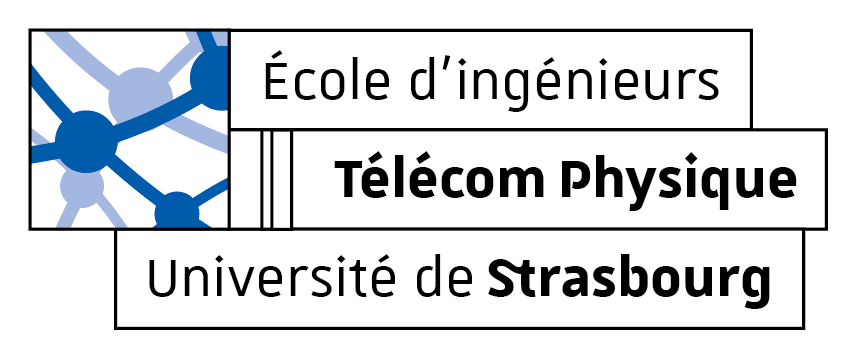
\includegraphics[scale=0.7]{logo_tps.png}
	\end{textblock*}


  \begin{sffamily}
    \begin{center}

      \vfill
      \textsc{\LARGE TPE Automatique et vision}\\[0.5cm]

      \textsc{\Large Asservissement visuel et commande}\\[1cm]

      % Title
      \HRule\\[0.4cm]
      {\huge \bfseries Rapport\\[0.4cm]}
      \HRule\\[1cm]

      \textsc{\Large Jonathan Plasse}\\[1cm]

      \textsc{\large Vendredi 15 Mars}



      \vfill

      % Bottom of the page
      {\large Année universitaire 2018 -- 2019}

    \end{center}
  \end{sffamily}
\end{titlepage}

\section*{Programmation}

	\subsection*{Update\_aoi}
		\subsubsection{Rôle}
			Cette fonction met à jour la position de l'imagette sur l'image afin de suivre l'objet.

		\subsubsection{Implantation}
			Tout d'abord, l'objet est approximé à une ellipse (en rouge) puis l'ellipse est considérée comme un rectangle (en bleu), on obtient finalement le rectangle (en noir) auquel est ajouté une marge de quelque pixels. L'imagette est ainsi obtenu.

			\begin{figure}[h]
			  \centering
		    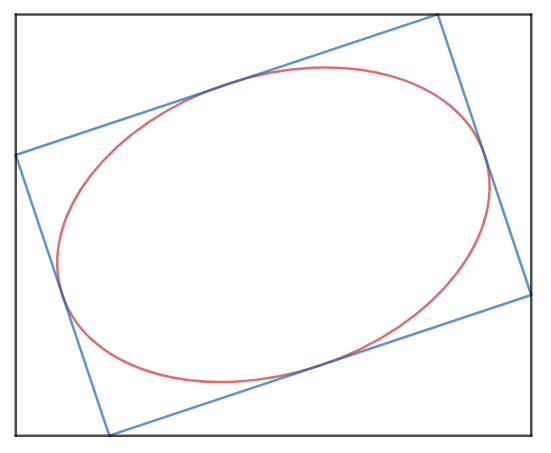
\includegraphics[width=0.5\textwidth]{imagette.png}
				\caption{Représentation de l'imagette}
			\end{figure}

			Si l'imagette dépasse de l'image elle est rogné pour tenir sur l'image.

	\subsection*{Moment}
		\subsubsection{Rôle}
			Cette fonction calcul les moments de l'imagette, avec ceux-ci l'objet contenu dans l'imagette peut être approximé par une ellipse.

		\subsubsection{Implantation}
			Les moments sont calculés avec cette formule.
			\[ m_{ij} = \iint_{D(t)} f(u, v) u^i v^i du dv \]

			On approxime cette double intégrale par une double somme.
			\[ m_{ij} = \sum_{i,j} f(u, v) u^i v^i \]

	\subsection*{Update\_mesure}
		\subsubsection{Rôle}
			Cette fonction calcul les translations et rotation que le robot doit éxécuter pour passer de l'image courante à l'image désiré.

		\subsubsection{Impantation}
			Pour faire ce calcul nous considérons deux points caractéristique de l'ellipse qui approxime l'objet. Ces points sont le centre $(cx, cy)$ et un sommet $(u,v)$ de l'ellipse.

			D'après les calculs fait en préparation le système suivant est obtenu.
			\[ A X=B \]
			\[
			\begin{pmatrix}
				cx_{ref}-u_0 & -(cy_{ref}-v_0)*\frac{\alpha_u}{\alpha_v} & \alpha_u & 0.0\\
				cy_{ref}-v_0 & (cx_{ref}-u_0)*\frac{\alpha_v}{\alpha_u} & 0.0 & \alpha_v\\
				u_{ref}-u_0 & -(v_{ref}-v_0)*\frac{\alpha_u}{\alpha_v} & \alpha_u & 0.0\\
				v_{ref}-v_0 & (u_{ref}-u_0)*\frac{\alpha_v}{\alpha_u} & 0.0 & \alpha_v\\
			\end{pmatrix}
			\begin{pmatrix}
				a_1\\
				a_2\\
				a_3\\
				a_4\\
			\end{pmatrix}
			=
			\begin{pmatrix}
				cx_{cur} - u_0\\
				cy_{cur} - v_0\\
				u_{cur} - u_0\\
				v_{cur} - v_0\\
			\end{pmatrix}
			\]

			\texttt{mathlib} est utilisé pour résoudre le système en faisant le calcul suivant.
			\[ X = A^{-1}B \]

			Les translations et rotation sont ensuite obtenu comme ceci.
			\[
			\begin{matrix}
				t_x & = & \dfrac{a_3z^*}{\sqrt{a_1^2+a_2^2}}\\
				t_y & = & \dfrac{a_4z^*}{\sqrt{a_1^2+a_2^2}}\\
				t_z & = & z^*(1-\dfrac{1}{\sqrt{a_1^2+a_2^2}})\\
				\alpha & = & \atantwo(a2,a1)\\
			\end{matrix}
			\]

	\subsection*{Commande}
		\subsubsection{Rôle}
			Cette fonction calcul la commande à envoyer au robot pour obtenir la position voulue.

		\subsubsection{Implantation}
			La commande à envoyer au robot est l'erreur entre la consigne et la mesure multipliée par un gain. Ici, nous avons les translations et rotation comme variables.

			La consigne est 0 pour les translations et rotation car nous voulons placer le robot de manière à obtenir l'image final.

			La mesure est les transalations et rotation calculées dans \texttt{Update\_mesure} $(t_x, t_y, t_z, \alpha)$.

			La commande donne.
			\[
			\begin{matrix}
				control_0 & = & -gain_t*t_x\\
				control_1 & = & -gain_t*t_y\\
			  control_2 & = & -gain_t*t_z\\
				control_3 & = & -gain_r*\alpha\\
			\end{matrix}
			\]
			
\end{document}
